\subsection{i}
Um die Anlagenkennlinie des Systems erstellen zu können, muss abschließend noch der
Gesamtdruckverlust $\Delta p_0$ aus der Summe der ermittelten Druckverluste berechnet werden.
Mit diesem wird entsprechend \autoref{eq:Kennlinie} die Kennlinie berechnet und visualisiert.
In \autoref{fig:Kenn_Mittel} ist die Kennlinie inklusive dem Betriebspunkt abgebildet.

\begin{equation}
    \label{eq:Kennlinie}
    \Delta p (\dot{V}) = \Delta p_0  \cdot \frac{\dot{V}}{ \dot{V_0} }
\end{equation}
\vspace{\baselineskip}
\begin{center}
    Gesamtdruckverlust $\Delta p_0 =p_r + p_{EW,WÜ} = 35048,28 Pa$\\
    Volumenstrom im Kollektorkreis $\dot{V_0} = 739,2\frac{l}{h}$
\end{center}
\vspace{\baselineskip}
\begin{figure}[H]
    \centering
    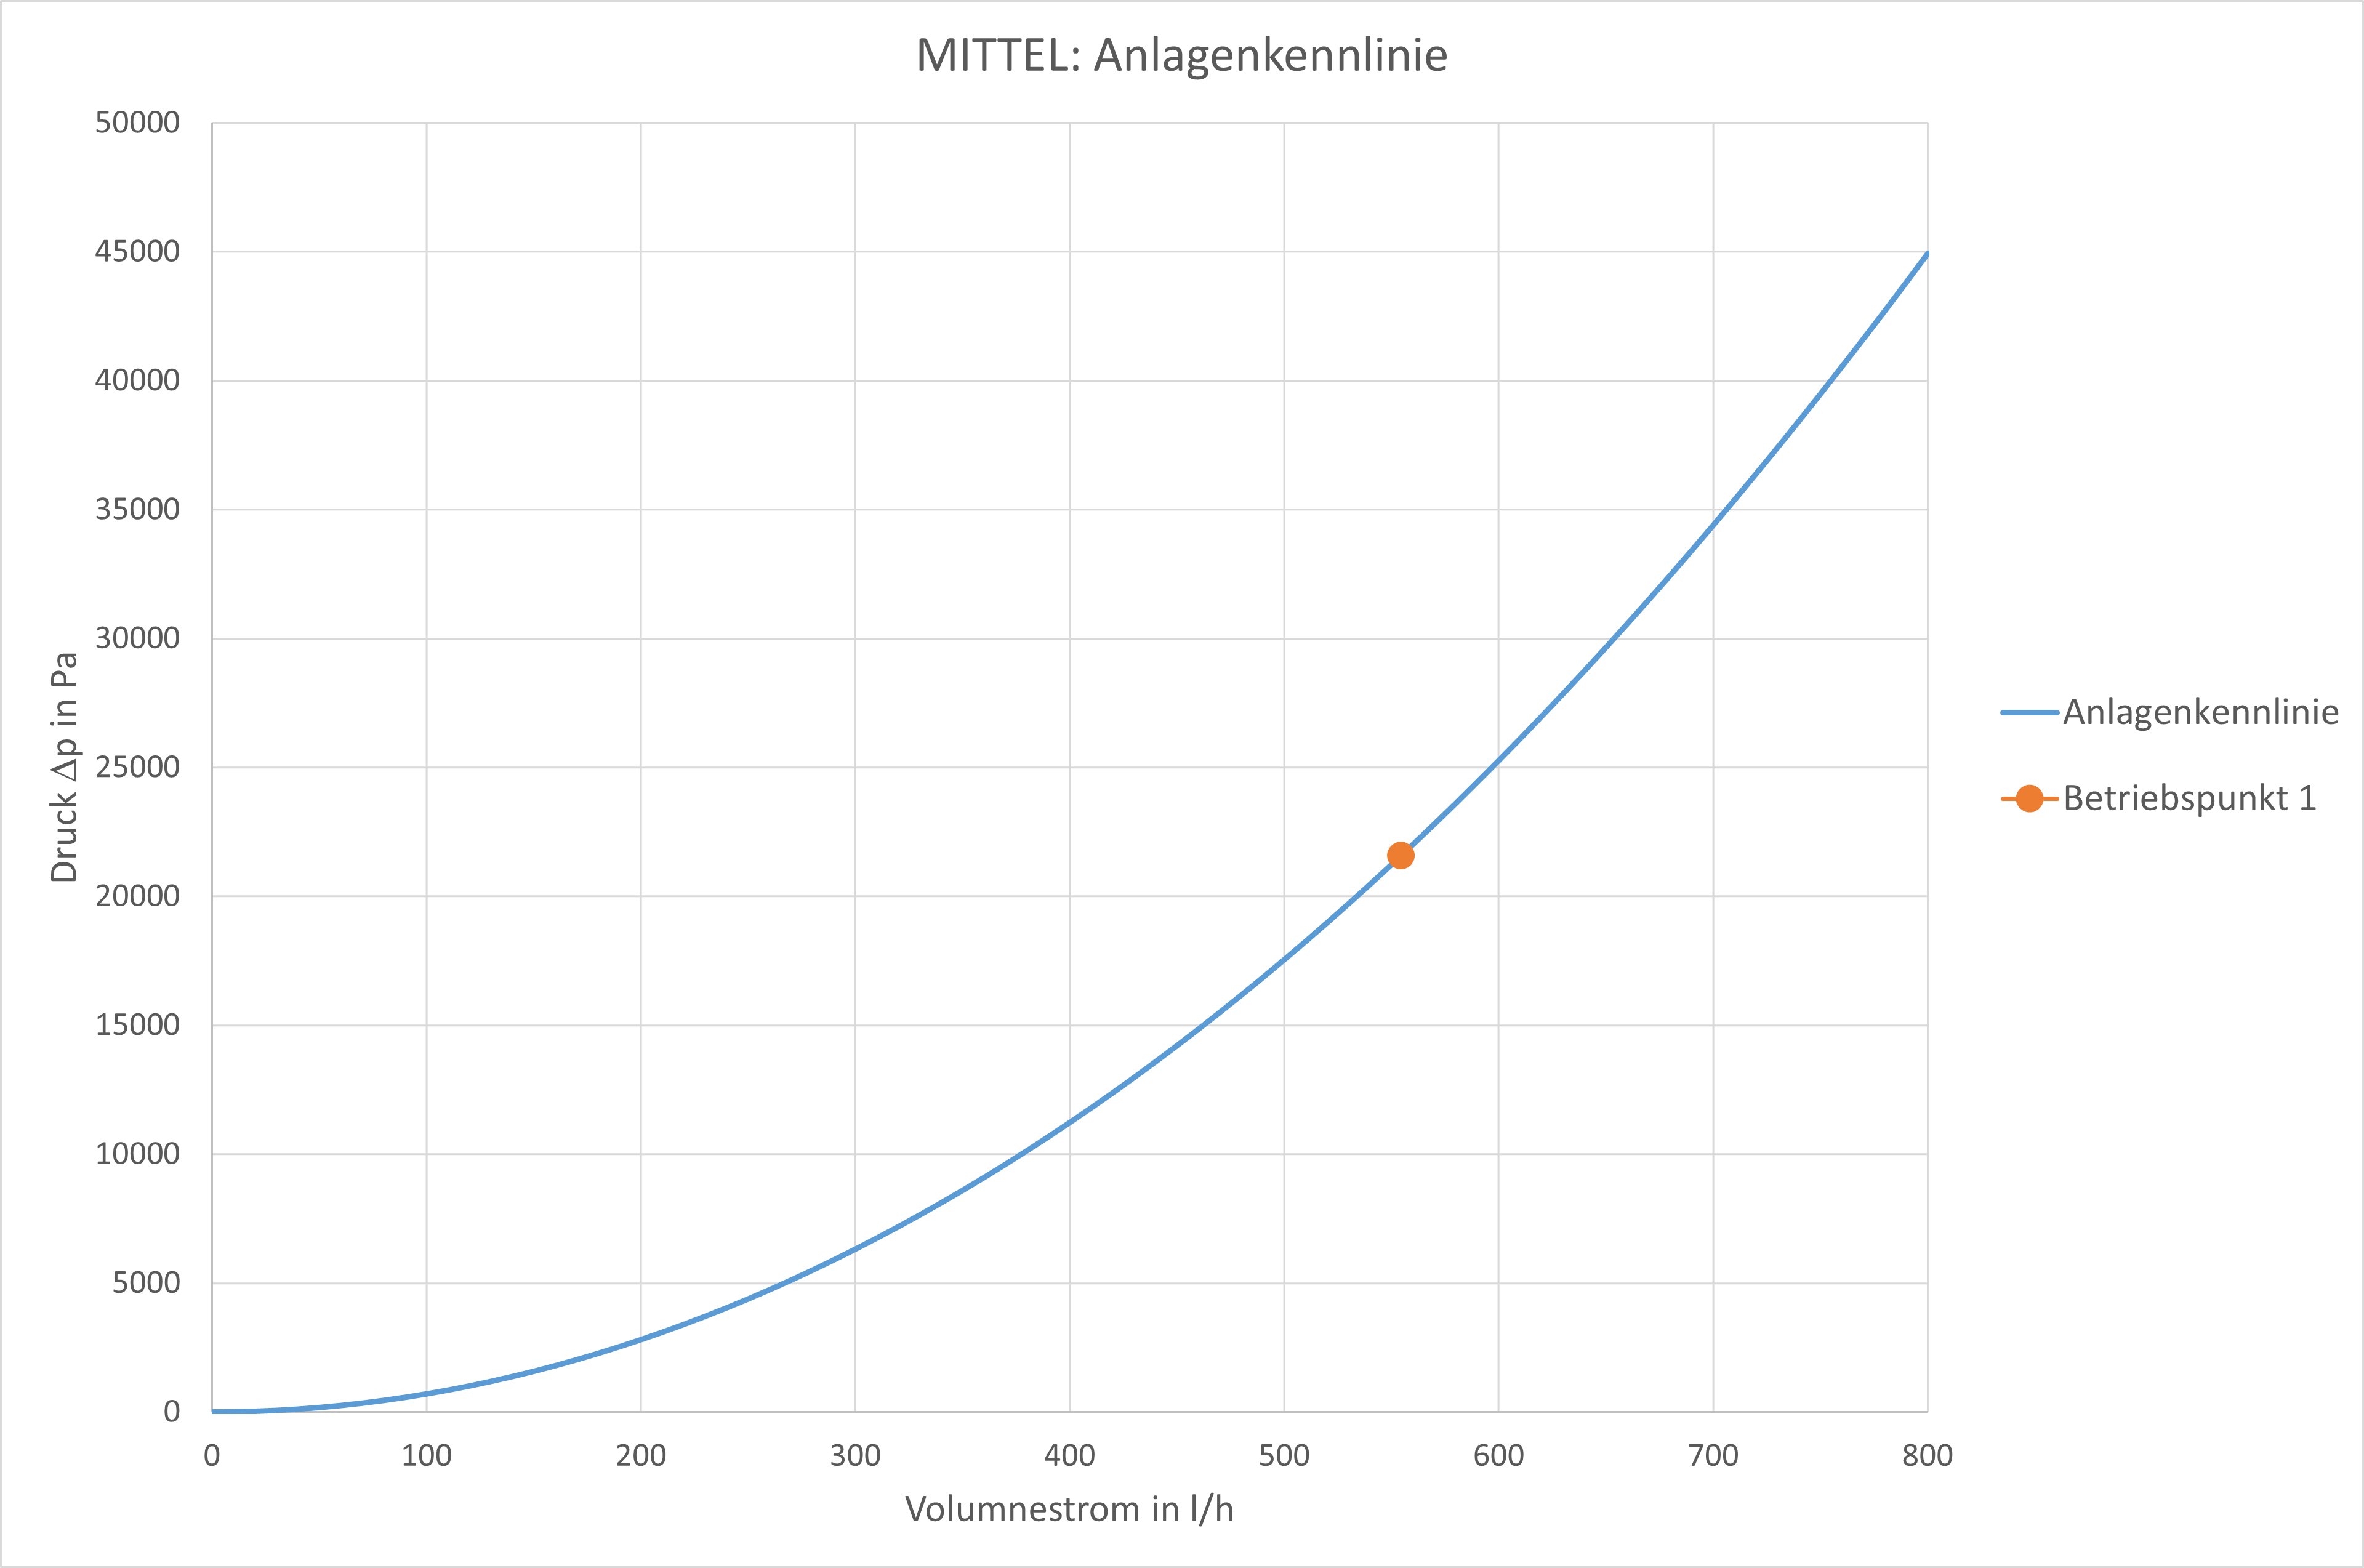
\includegraphics[width=1\textwidth]{Abbildungen/Kennlinie-Mittel.png}
    \caption{Anlagenkennlinie des gemittelten Systems}
    \label{fig:Kenn_Mittel}
\end{figure}